\section{Methodology}
\label{sec:ch5-methodology}

This section describes the study design and structure of our three sessions. We then outline the design tools and procedures, followed by session-level reporting (Layer~0), and finally the multi-layered analysis of the shared empirical corpus (Layers~1---3).

\subsection{Study Design: Three Expert Design Sessions}
\label{subsec:ch5-study-design}
The sessions were designed as interrelated phases of a single, evolving inquiry, each building on the previous one. Session~1 surfaced the breadth of biophilic experiential qualities diminished or absent indoors. Session~2 examined their spatial and material translation. Session~3 focused on sound as a biophilic design material.

\begin{maintable}[tbp]
\caption{Overview of experts in the three design sessions. Experts' background represents their primary areas of practice.}
\label{tab:expert-demographics}

\fontsize{8.4}{10.0}\selectfont
\setlength{\tabcolsep}{3pt}
\renewcommand{\arraystretch}{1.06}

\begin{tabularx}{\linewidth}{@{}p{.26\linewidth} p{.23\linewidth} Y@{}}
\toprule
\textbf{Session} & \textbf{Role} & \textbf{Background / Expertise} \\
\midrule

Session~1 Benthem Crouwel Architects &
Senior Architect &
Large-scale public and commercial buildings \\

&
Designer &
Concept development \\

&
Designer &
3D visualisations and spatial representation \\

&
Architect &
Design and spatial planning \\

\midrule

Session~2 Up Architecture &
Senior Architect &
Sustainability \\

&
Senior Architect &
Interior architecture and renovation \\

&
Senior Architect &
Building envelopes and exteriors \\

&
Architect &
Interior design \\

\midrule

Session~3 Makers of Sustainable Spaces &
Designer &
Green design \\

&
Designer &
Green design \\

&
Designer &
Green design \\

&
Designer &
Green design \\

&
Design Communications &
Green design \\

\bottomrule
\end{tabularx}

\Description{A table summarising the experts who participated in the three design sessions, listing each participant along with their primary area or areas of professional practice and background.}
\end{maintable}

\paragraph{Experts}
\label{subsubsec:ch5-experts}
We engaged architects and designers from established architecture practices and design studios. Each session involved a different group of experts and was designed as a distinct yet connected exploration rather than a longitudinal study. This introduced variation in expertise and design reasoning, enabling identification of recurring patterns across independently generated concepts. We worked with practising architects and designers as participants, to access forms of spatial and experiential reasoning that are typically under-articulated in technology-led approaches. Architects are trained to think in terms of atmosphere, materiality, environmental variation, and spatial behaviour over time, and are therefore well positioned to speculate on how biophilic qualities might be composed at architectural scale. This expertise enabled the sessions to elicit generative imaginaries and design logics, which informed the articulation of the biophilic interaction design framework. This decision foregrounds a particular type of knowledge: how interaction is imagined and structured from a design perspective, rather than how it is experienced in everyday use. Experts were recruited through professional networks and prior research collaborations. All sessions were conducted in English. A summary of expert backgrounds and roles is provided in \autoref{tab:expert-demographics}. Ethical approval was obtained from our institutional review board. All experts also provided verbal and written consent.




\begin{mainfigure}[tbp]
    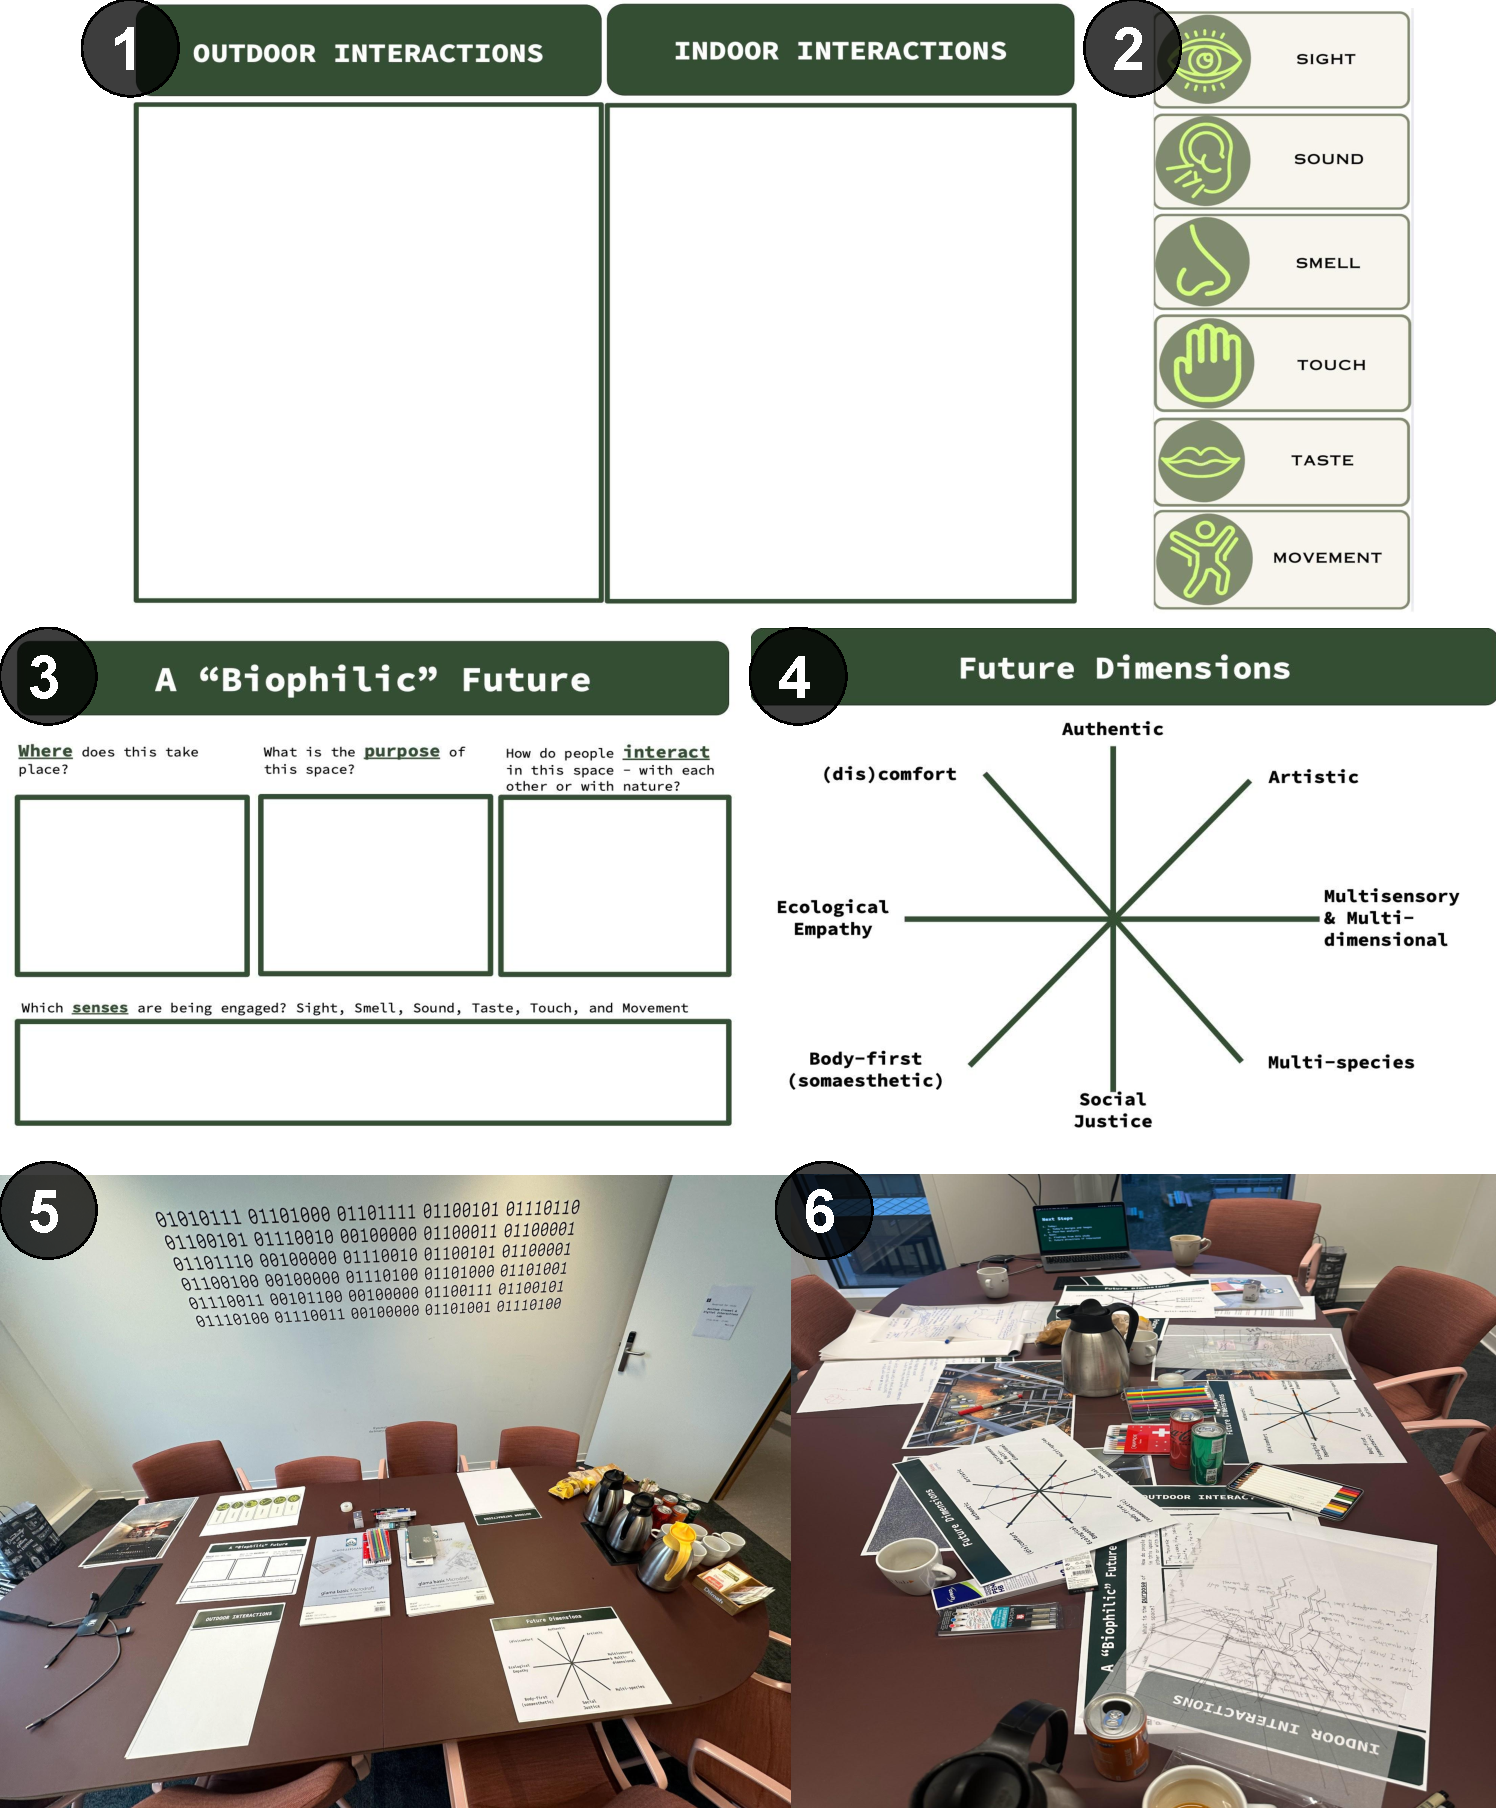
\includegraphics[width=\linewidth]{images/methodology/dis26-materials.pdf}
    \caption{Overview of the design tools used across the three expert sessions. From left to right: (1) an outdoor–indoor interactions template used to note outdoor experiences and reflect on how they change indoors; (2) a senses reminder sheet for multisensory design, listing six sensory modalities (sight, sound, smell, touch, taste, and movement); (3) the \emph{Biophilic Things of the Future} template, adapted from the \emph{The Thing From The Future} method, used to scaffold speculative design discussion around spatial context, interaction, and sensory modalities; (4) a circular mapping artefact with eight biophilic dimensions for future smart buildings~\cite{rao2025designing}, used for reflection; and (5–6) examples of session materials, setup, and after design activities.} 
    \label{fig:design-tools}
    \Description{An overview of the design tools used across the three expert design sessions. From left to right, the figure shows: an outdoor–indoor interactions template for reflecting on changes in experience; a multisensory reminder sheet listing six sensory modalities; a Biophilic Things of the Future template used to scaffold speculative design; a circular mapping artefact representing eight biophilic dimensions; and photographs of session materials, setup, and post-design activities.}
\end{mainfigure}

\subsection{Session Procedure and Design Tools}
\label{subsec:ch5-session-procedure}
Across all sessions, we followed a shared structure designed to foreground lived experience while supporting speculative exploration. Each session began with an introduction and consent, followed by a short outdoor walk\sidenote{Walks took place at a local permaculture garden, coastal dunes, and alongside a river.} used to provide a mental reset after the working day (rather than as a prompt for reflecting on specific outdoor environments or experiences). A guided round-table discussion then invited experts to articulate how biophilic experience is perceived and interpreted, with prompts varying by session focus. Details are provided in \autoref{sec:ch5-overview}.

Each session then included a speculative group design activity using the \emph{Biophilic Things of the Future}, inspired by the \emph{The Thing From The Future} method~\cite{candy2018gaming}\sidenote{\url{https://ncsu-libraries.github.io/the-thing-from-the-future/}} (and used in speculative design thinking e.g. \cite{becsevli2024smell, becsevli2025sonarios}). The template scaffolded discussion around spatial context, purpose, interaction, and sensory modalities. Additional materials (multisensory prompts, indoor imagery, tracing paper, sketching tools) supported situated and iterative design exploration. Activities were think-aloud exercises and experts were instructed to ignore technical, regulatory, or budgetary constraints.

Each session concluded with a reflective discussion in which groups presented their concepts. Reflection was supported by a circular mapping artefact based on previously established dimensions of biophilic experience in indoor environments~\cite{rao2025designing}, which experts used to discuss which experiential qualities their concepts amplified, transformed, or left unaddressed. An overview of the design tools and artefacts is in Figure~\ref{fig:design-tools}.

The workshop structure, prompts, and tools supported articulation rather than prescribing outcomes. Prompts directed attention to aspects of biophilic experience (e.g. perception, spatial translation, sound) without specifying concepts, values, or interaction logics. Design templates and artefacts provided a shared language for externalising and comparing ideas that might otherwise remain tacit. The resulting material reflects both expert-generated concepts and the structuring role of the workshop: articulation was guided, but the content and direction of ideas were driven by the experts.


\subsection{Data Collection and Processing}
\label{subsec:ch5-data-processing}
The dataset comprised audio recordings of group discussions, transcripts, completed design templates, sketches, photographs of artefacts, and reflection maps produced during each session. All audio recordings were transcribed. Visual materials were digitised and linked to corresponding transcript segments. Data were organised per session and per design group to preserve context.


\subsection{Data Analysis}
\label{sec:ch5-data-analysis}
Our analysis moved from descriptive accounts (Layer~0) to higher-level abstraction (Layers~1---3), examining what was imagined, why it was valued, and how it was articulated as interaction over time (\autoref{fig:study-overview}). The unit of analysis varied by layer. In Layer~1, it was \emph{each statement associated with a design concept}, capturing how experts described or specified aspects of a proposed idea. In Layer~2, it was a \emph{segment of evaluative reasoning}, where experts articulated preferences, constraints, or judgements. In Layer~3, it was an \emph{interaction episode} describing relations between bodily action, environmental condition, and experiential consequence. Analysis was led by the first author, with regular discussions with the third author to review decisions, resolve ambiguities, and finalise constructs.

\begin{mainfigure}[tbp]
    \centering
    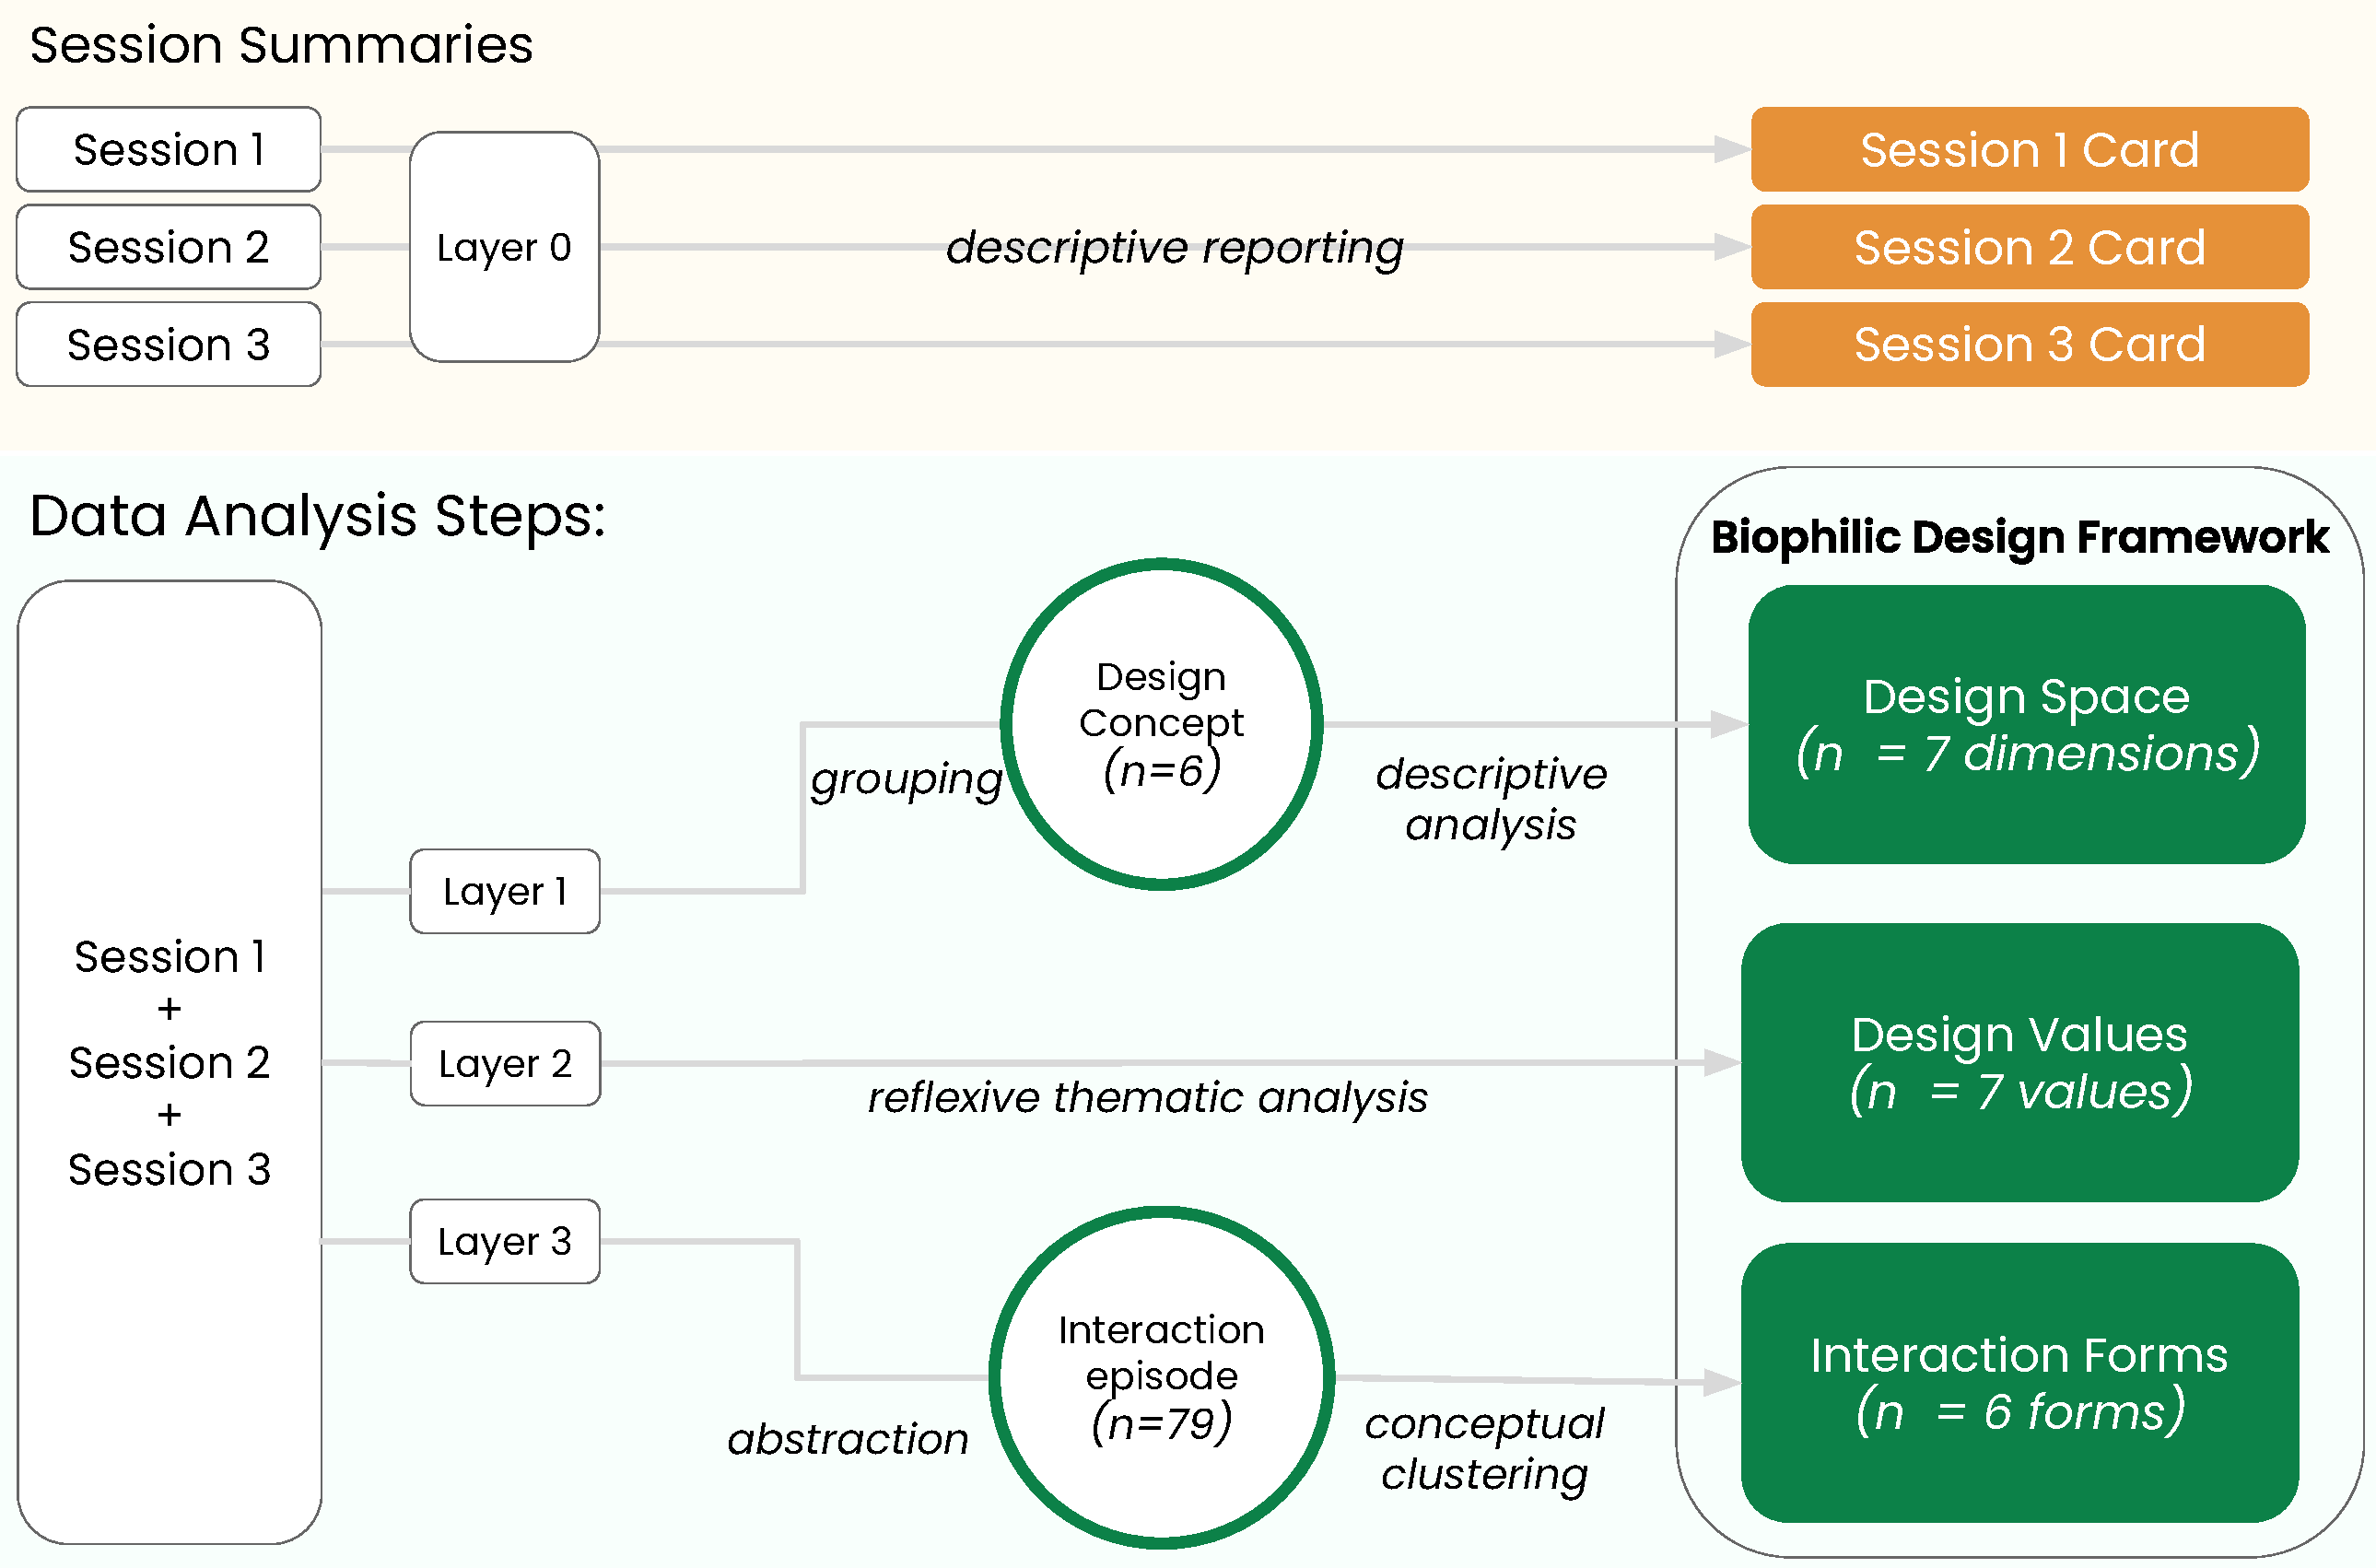
\includegraphics[width=\linewidth]{images/methodology/methodology-overview.pdf}
    \caption{Multi-layered analysis of three expert design sessions. Layer 0 provides descriptive session-level reporting; Layer 1 maps the biophilic design space through descriptive content analysis; Layer 2 surfaces biophilic interaction design values via reflexive thematic analysis; and Layer 3 abstracts recurrent interaction episodes into biophilic interaction forms. Layers 1–3 draw on the full empirical corpus, while Layer 0 documents each session independently.}
    \Description{A diagram illustrating the multi-layered analysis of the three expert design sessions. The figure shows four analytic layers: Layer 0 presents descriptive session-level reporting; Layer 1 maps the biophilic design space using descriptive content analysis; Layer 2 identifies biophilic interaction design values through reflexive thematic analysis; and Layer 3 abstracts recurring interaction episodes into biophilic interaction forms. Layers 1–3 draw on the full dataset, while Layer 0 documents each session independently.}
    \label{fig:study-overview}
\end{mainfigure}


\paragraph{Layer 0: Session-Level Reporting}
\label{subsec:ch5-layer0}
We first descriptively documented each session through session-level summaries to make visible what was discussed and produced. These accounts do not involve cross-session synthesis or researcher interpretation. To ensure consistency across sessions, we developed a structured reporting template that guided what was extracted from each session. Using this template, we recorded the experiential aim, relevant metadata (e.g. number of experts, duration, date), selected the most complete and representative visual artefacts produced (often from a larger set), and summarised key remarks and outcomes, including how each session informed the framing of the subsequent one. Each session is presented through a visual session card accompanied by a brief account.


\paragraph{Layer 1 — Design Space Dimensions (RQ1)}
\label{subsec:ch5-layer1}
This layer maps the design space of future biophilic experiences imagined for indoor environments (RQ1). It shares what qualities were imagined and how different experiential configurations were articulated across the expert design sessions. Each session produced speculative proposals, treated here as a \emph{design concept}, used solely as an organising anchor. All transcripts were reviewed and discussion segments were tagged by the design concept they referred to, resulting in six design concepts (see \autoref{tab:codebook-design-concepts}). We then analysed the statements associated with the design concepts using Krippendorff~\cite{krippendorff2018content}'s descriptive content analysis. The first author developed an initial codebook through a preliminary reading, identifying candidate dimensions and codes based on how experts specified biophilic experiences. The first author then defined and applied these to a subset of the data to test their clarity and consistency. Analytic decisions regarding code definitions, naming, and organisation were discussed with the third author to ensure clarity and conceptual coherence. The refined codebook was subsequently used to code the full dataset. The final codebook contained seven descriptive dimensions with associated codes that together capture how biophilic interaction concepts were articulated (e.g. \texttt{sensory modality}, \texttt{spatial context}, \texttt{interaction type}, see \autoref{tab:layer1-codebook}).

\paragraph{Layer 2 — Design Values (RQ2)}
\label{subsec:ch5-layer2}
We did reflexive thematic analysis following Braun and Clarke~\cite{braun2023thematic,braun2022conceptual}, focusing on the value orientations that shaped how experts reasoned about the translation of biophilic experiences into indoor environments. The first author generated $48$ initial codes capturing statements that articulated limits (e.g. ``this shouldn’t be too much''), expressed concern (e.g. ``we don’t want it to become a gimmick''), or framed qualities as needing to be optional, subtle, or ambiguous. Example codes are \textit{optional rather than imposed}, \textit{avoid gimmickry}, \textit{respect context and atmosphere}, and \textit{retain ecological meaning rather than simulate superficially}. Codes that expressed similar normative orientations (e.g. restraint, authenticity, contextual sensitivity) were grouped into seven distinct themes\sidenote{We did not calculate inter-coder agreement, as Layer~2 was conducted as reflexive thematic analysis, where analytic rigour is established through iterative engagement with the data, transparency of interpretation, and conceptual clarity rather than coder convergence.} called biophilic design values. 

\begin{mainfigure}[!ht]
  \centering
  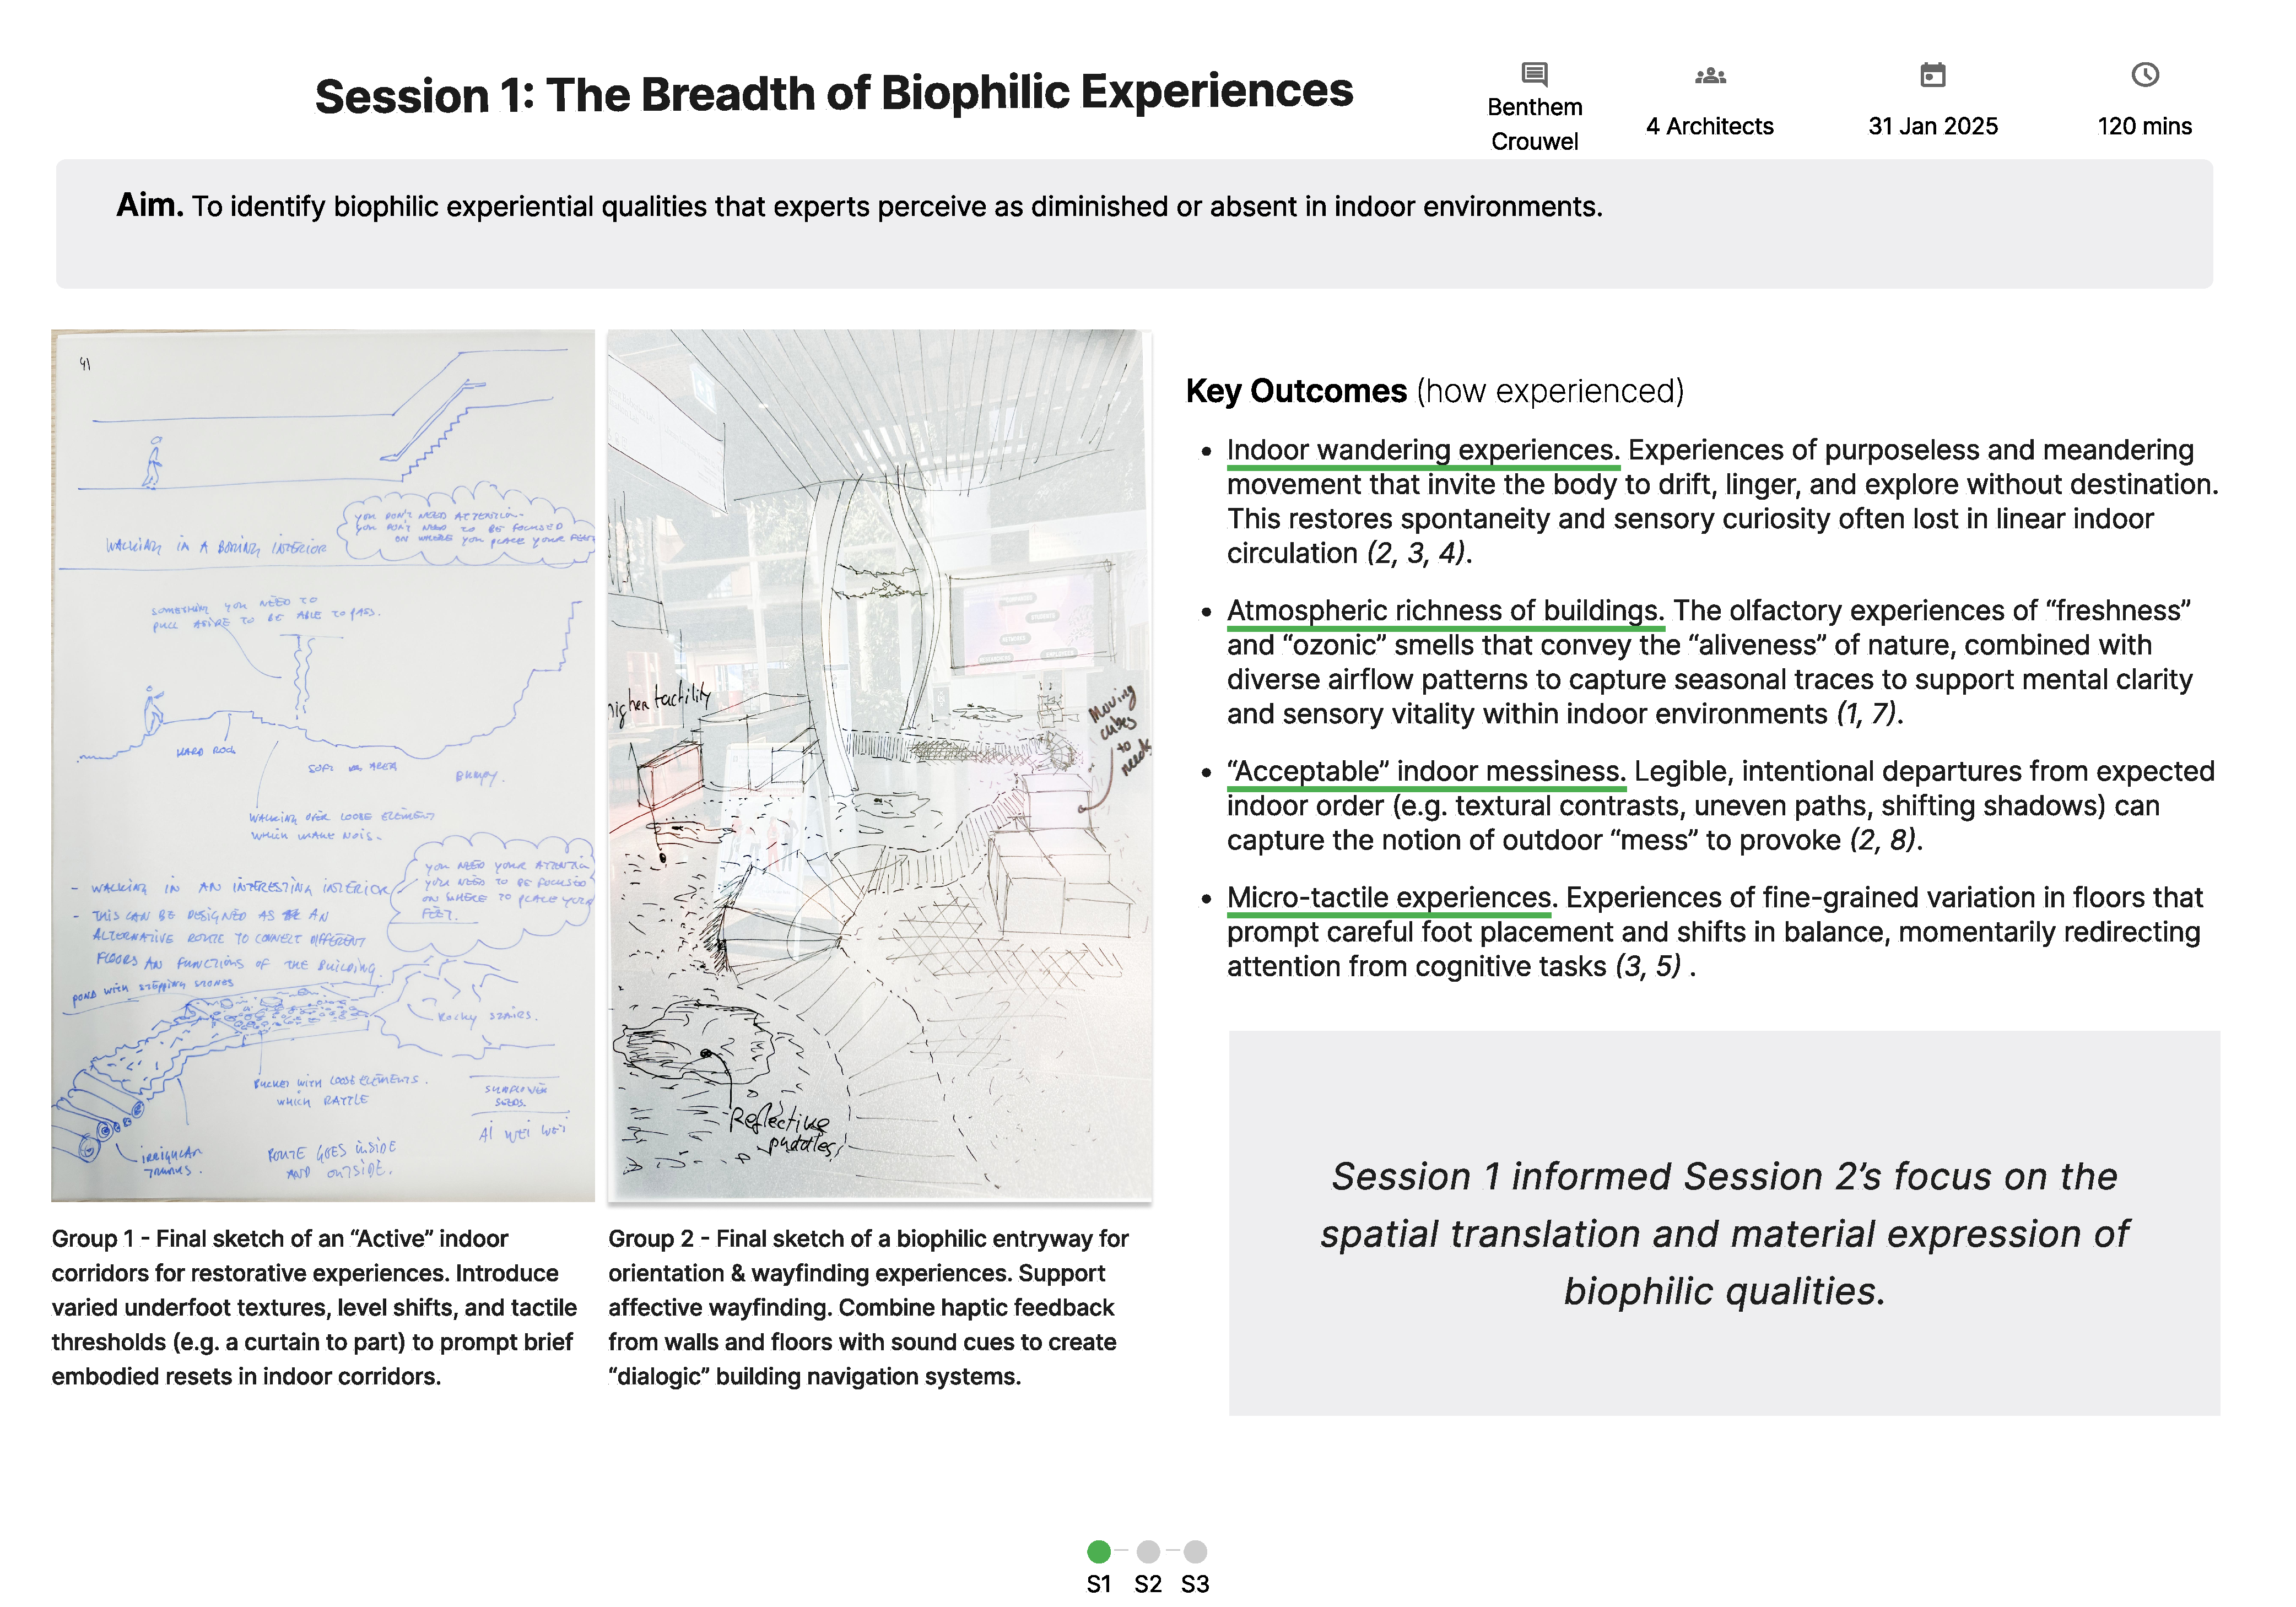
\includegraphics[width=\linewidth]{images/l0/final-w1-version2 (3).pdf}
  \caption{Session~1 card summarising the session aim, structure, selected sketches, and a condensed overview of session-level experiential outcomes related to how biophilic experience was perceived and described.}
  \Description{A session card summarising Session 1, showing the session aim, structure, selected expert sketches, and a brief overview of session-level experiential outcomes related to how biophilic experience was perceived and described.}
  \label{fig:w1-card}
\end{mainfigure}

\paragraph{Layer 3 — Biophilic Interaction Forms (RQ3)}
\label{subsec:ch5-layer3}
Finally, we developed biophilic interaction forms that capture recurring ways in which experts imagined occupants interacting with future biophilic environments. Biophilic interaction refers to bodily interaction with technologically mediated indoor environments, occurring through bodily action, sensing, and environmental response over time. We identified $79$ \emph{interaction episodes} describing relations between bodily action, environmental condition, and experiential consequence (e.g. slowing down in response to sound). Episodes were abstracted by removing context-specific details (e.g. particular materials, room types, or firm-specific language) while preserving interaction logic, enabling comparison across concepts. For example, an episode describing slowed movement through layered materials was abstracted as \textit{irregular pathway, continuous bodily adjustment, somatic awareness}. Next, abstractions were iteratively compared and clustered based on shared interaction logics (e.g. presence, movement, touch),  resulting in nine initial interaction forms. These were iteratively reviewed, merged, and refined through discussions between the first and third author to resolve overlaps and sharpen distinctions, resulting in six final interaction forms.



\paragraph{Summary.}
Layer~1 maps \emph{what} kinds of biophilic interaction concepts were imagined across the sessions; Layer~2 examines \emph{why} particular experiential orientations and boundaries shaped these concepts; and Layer~3 articulates \emph{how} interaction was envisioned through recurring patterns of bodily interaction with technology-mediated environments.
